\section{Single Robot Method Comparison}
\label{sec:04_tdoaSingle}

For comparability of the results, the same measurements are taken into
account to analyse the \ac{TDOA} methods.
Part of the channel inputs of the whistle signal used in this section is plotted
in \ref{fig:04_tdoaSignal}.
Here, the sound source is placed -33.7\si{\degree} on the right front
of the robot with 4.5\si{m} distance.
In \cref{fig:04_tdoaSignal} we see the first samples of this whistle signal.
% -------------------------------------------------------------
\begin{figure}[ht]
	\centering
		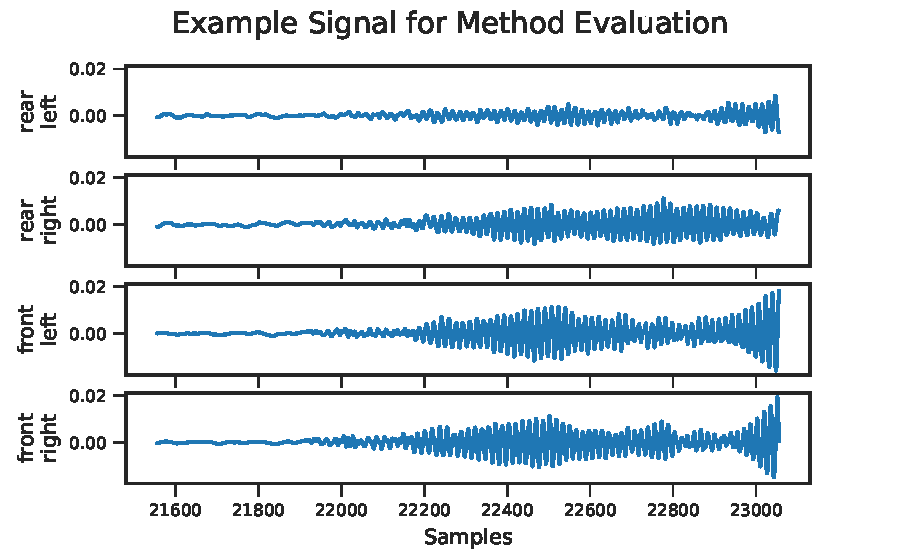
\includegraphics[]{figures/evaluation/cc_frontRight_1_signal}
	\caption{Signal start section of a whistle sound recorded from front right.}
	\label{fig:04_tdoaSignal}
\end{figure}
% -------------------------------------------------------------

The signal start index to choose the frame is detected with the algorithm introduced in
\change[]{which index? Explain better.} \cref{sec:03_signalStartDetection}.
A frame size is set to 256 samples and is selected around the start index for
\ac{CC} and \ac{GCC}.
For the phase method the first frame with the same maximal frequency is chosen.

\subsection{Cross Correlation}
\label{subsec:04_ccSingle}
% -------------------------------------------------------------

To visualize the result of the \ac{CC}, the correlations are plotted in
\cref{fig:04_cc}. For $R_{23}$ and $R_{13}$ the peak is clearly traceable.
However, for the other \ac{CC} the problem mentioned in \cref{sec:02_cc}
arises and the maximum peak does not differ much from the other tips.

\begin{figure}[ht]
	\centering
		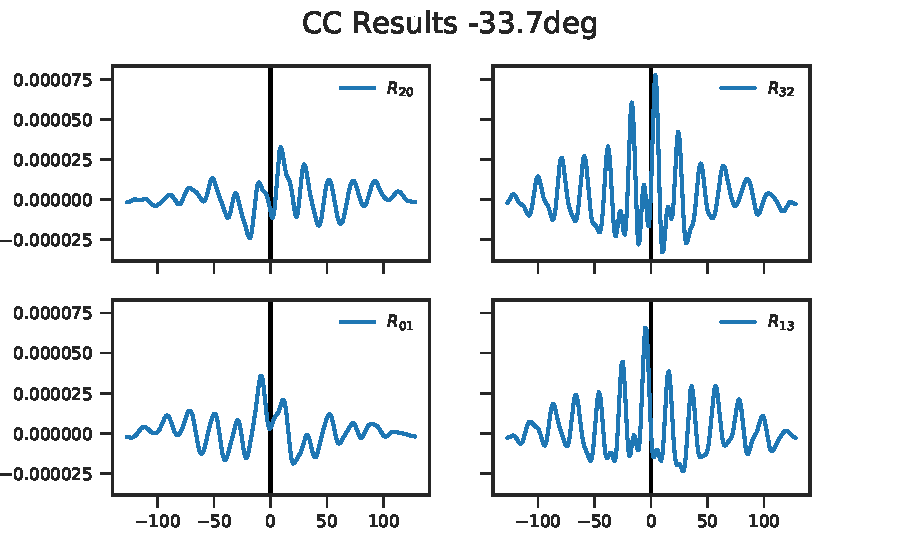
\includegraphics[]{figures/evaluation/cc_frontRight_1}
	\caption{Cross correlation results of signal from front right.}
	\label{fig:04_cc}
\end{figure}

\btline{ht}{1.2}
\btab{|c|c|c|c|c|}
\hline
Base Channel & Next Channel & Delay & Candidate (-) & Candidate (+)\\
\hline
0 & 1 & -8.25 & -144.9 & -35.1\\
\hline
1 & 3 & -4.59 & -17.4 & 78.6\\
\hline
2 & 0 & 9.16 & -30.6 & -30.6\\
\hline
3 & 2 & 3.94 & -150.2 & -29.8\\
\hline
\etab
\et{Cross correlation delay results of singal from front right.}{04_cc}

According to the delays in \cref{tab:04_cc}, the final result of the \ac{CC}
is -26.9\si{\degree} with an error of 6.8\si{\degree}.
Taking a closer look at the delay between channel 2 and channel 0, we see that
the delay is larger than the expected maximal delay of 6.85 samples
% -------------------------------------------------------------
\subsection{Generalized Cross Correlation}
\label{subsec:04_gccSingle}
% -------------------------------------------------------------
\Cref{fig:04_gcc} demonstrates the results of the \ac{GCC} of the received signal.
The single delays and the resulting angle candidates are listed in \cref{tab:04_gcc}
and lead to a final direction of -30.8\si{\degree} with an error of 2.85\si{\degree}.
We can see that the peaks of the \ac{GCC} are better to detect than the peaks of the
\ac{CC}.
% -------------------------------------------------------------
\begin{figure}[ht]
	\centering
		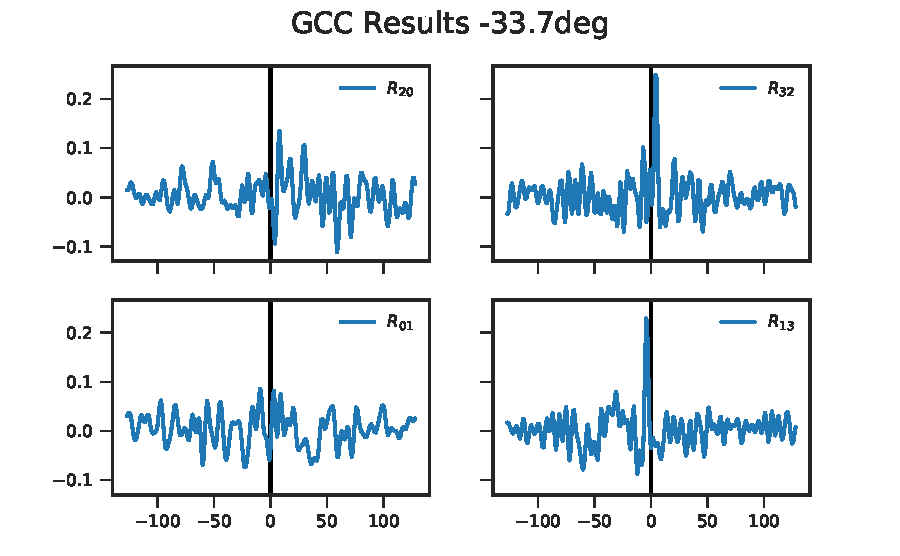
\includegraphics[]{figures/evaluation/gcc_frontRight_1}
	\caption{Generalized cross correlation results of signal from front right.}
	\label{fig:04_gcc}
\end{figure}
% -------------------------------------------------------------
\btline{ht}{1.2}
\btab{|c|c|c|c|c|}
\hline
Base Channel & Next Channel & Delay & Candidate (-) & Candidate (+)\\
\hline
0 & 1 & -8.96 & -141.3 & -38.7\\
\hline
1 & 3 & -3.85 & -25.2 & 86.4\\
\hline
2 & 0 & 7.71 & -30.6 & -30.6\\
\hline
3 & 2 & 4.38 & -146.6 & -33.4\\
\hline
\etab
\et{Generalized cross correlation delay results of singal from front right}{04_gcc}
% -------------------------------------------------------------
\subsection{Phase Difference}
\label{subsec:04_phaseSingle}

For the source direction detection with phase difference, a smaller frame
size of 62 samples is set.
Previously, two cases were introduced in \cref{subsec:03_phase} where either a
fixed frequency is focused on or the frequency with maximal magnitude is
taken for reference.

First, the result of the dynamically selected frequency is presented.
As stated in the implementation chapter, the frame is chosen where the
frequencies of the maximal amplitudes coincides for all channel which is
at 2756,25\si{\hertz}.
In the upper plot of \cref{fig:04_phaseSingle} one sees the received samples which
will be transformed into frequency domain by \ac{FFT} and using a Hann window.
The resulting phases and amplitudes are listed in \cref{tab:04_phaseSingle}.
For comprehensibility, the determined frequency information visualized by
wave signals with these phases and amplitudes
in the lower subplot of \cref{fig:04_phaseSingle}.
Due to the larger distance between channels 0 and 1, the phase difference
information is neglected.
Outcome from the applied phase differences is -29,2\si{\degree} by the combination of
-17,6\si{\degree}, -30,6\si{\degree} and -39,3\si{\degree}.
% -------------------------------------------------------------
\btline{ht}{1.2}
\btab{|c|c|c|}
\hline
Channel & Phase [\si{\deg}] & Amplitude\\
\hline
0 & -1,55 & 0,00144\\
\hline
1 & -177,7 & 0,00287\\
\hline
2 & 173,4 & 0,00279\\
\hline
3 & -75,0 & 0,00372\\
\hline
\etab
\et{Phase and amplitude of frame signals with 2756,25Hz}{04_phaseSingle}
% -------------------------------------------------------------
\btline{ht}{1.2}
\btab{|c|c|c|c|c|}
\hline
Base Channel & Next Channel & Phase Difference & Candidate (-) & Candidate (+)\\
& & [\si{\deg}] & [\si{\deg}] & [\si{\deg}] \\
\hline
0 & 1 & 176,2 & 33,07 & 146,9\\
\hline
1 & 3 & -102,7 & -17,6 & 78,8\\
\hline
2 & 0 & 173,4 & -30,6 & -30,6\\
\hline
3 & 2 & 113,1 & -140,7 & -39,3\\
\hline
\etab
\et{Phase differences and resulting direction candidates of example data with phase method}{04_phaseDiffSingle}
% -------------------------------------------------------------
\begin{figure}[ht]
	\centering
		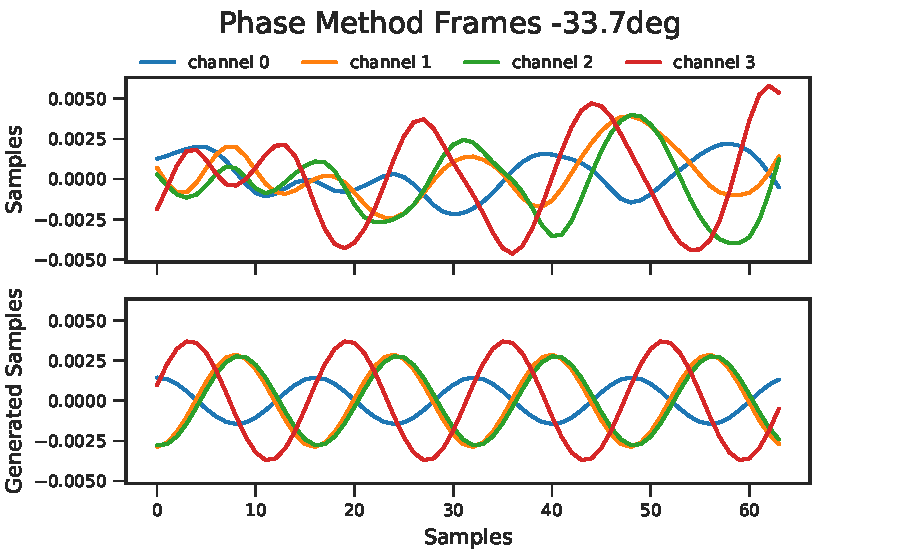
\includegraphics[]{figures/evaluation/phase_cos}
	\caption{Frames used for the direction detection by phase method.}
	\label{fig:04_phaseSingle}
\end{figure}
% -------------------------------------------------------------

Secondly, the frequency to examine $f_c$ is set to the first represented frequency
larger than 2400\si{\hertz} which is 2411,72\si{\hertz} at a \ac{FFT} length
of 256.
At this frequency, outcome of the direction candidates listed in \cref{tab:04_fixedFreqResult}
with the considered delays is -30,0\si{\degree}.
% -------------------------------------------------------------
\btline{ht}{1.2}
\btab{|c|c|c|c|c|}
\hline
Base Channel & Next Channel & Phase Difference & Candidate (-) & Candidate (+)\\
& & [\si{\deg}] & [\si{\deg}] & [\si{\deg}] \\
\hline
1 & 3 & -72,8 & -26,7 & 87,9\\
\hline
2 & 0 & 167,5 & -30,6 & -30,6\\
\hline
3 & 2 & 84,6 & -147,2 & -32,8\\
\hline
\etab
\et{Resulting candidates of phase difference method with fixed frequency
	2411,72Hz of example measurement from front right
	(-33,3\si{\degree})}{04_fixedFreqResult}
% -------------------------------------------------------------